\documentclass[12pt]{amsart}
\pagestyle{empty}
\usepackage[hmargin=1in,vmargin=1in]{geometry}
\usepackage{url,  mathrsfs}
\usepackage{hyperref}
\usepackage{fancyhdr} 
\usepackage[T1]{fontenc}


\usepackage{url,  mathrsfs}
\usepackage{hyperref}
\usepackage{amsmath}
\usepackage{graphicx,  epstopdf}
\usepackage{subfig}
\usepackage{color}
\usepackage{bbm}
\usepackage{subfloat}
\usepackage[draft]{fixme}
\usepackage{bm} 
\usepackage{bbm} 
\usepackage{epigraph}
\usepackage{endnotes}
\usepackage{ifpdf}
\usepackage{array}

\usepackage{multicol}
\usepackage{multirow}
\usepackage{graphicx}
\usepackage{tikz}

\newcommand{\A}{\mathbb{A}}
\newcommand{\Q}{\mathbb{Q}}
\newcommand{\N}{\mathbb{N}}
\newcommand{\Z}{\mathbb{Z}}
\newcommand{\R}{\mathbb{R}}
\newcommand{\F}{\mathbb{F}}
\newcommand{\C}{\mathbb{C}}
\renewcommand{\P}{\mathbb{P}}
\newcommand{\I}{\mathcal{I}}
\newcommand{\V}{\mathcal{V}}
\newcommand{\cH}{\mathcal{H}}
\newcommand{\ol}{\overline}
\newcommand{\J}{\mathcal{J}}
\newcommand{\X}{\mathcal{X}}
\theoremstyle{definition}
\newtheorem{prob}{Problem}
\newtheorem{extraProb}{Extra Problem}

\DeclareMathOperator{\conv}{conv}
\DeclareMathOperator{\cone}{cone}
\DeclareMathOperator{\ext}{ext}




\begin{document}
 \thispagestyle{empty}
\begin{center} {\large \textbf{Math 380 -- Homework  3}} \smallskip \\ 
Due on Thursday, April 23\ \\ \ \\
 \end{center}

You are welcome to talk with other students in the class about problems but should write up solutions on your own. 
Solutions can be handwritten or typed but need to be legible and submitted via Gradescope by the end of the day 
on Thursday. You should justify all your answers in order to receive full credit.  
\bigskip 

\begin{flushleft}

{\bf Good practice problems} (not to be turned in): \\

CLO Section 2.2, Exercises 1, 7, 8\\
CLO Section 2.3, Exercises 1, 2, 4, 6 \\
CLO Section 2.4, Exercises 4, 5, 9, 10\\ \ \\
\bigskip 




\begin{prob} CLO \S2.2, Exercises 11 and 12\\
\end{prob}
\bigskip 

\paragraph{Problem 11} Let $>$ be a monomial order on $k[x_1,\dots,x_n]$. \begin{enumerate}
    \item[a.] For any $f \in k[x_1,\dots,x_n]$ and any monomial $m$, we have $\text{LT}(m\cdot f) = m\cdot \text{LT}(f)$. We can write $f$ as a finite $k$-linear combination of monomials: \[
    f = \sum_{\alpha \in A} c_\alpha x^\alpha.
    \]
    Let $\alpha_m$ denote the leading monomial of $f$ so that we have $\alpha_m \ge \alpha$ for all $\alpha \in A$. Also, let $m = x^\gamma$ for some $\gamma \in \mathbb Z^n_{\ge 0}$. Then, by the definition of leading term, we have \[m\cdot \text{LT}(f)=m\cdot c_{\alpha_m}x^{\alpha_m} = c_{\alpha_m} x^{\alpha_m+\gamma}.\]
    We can also write \[m \cdot f = x^\gamma \sum_{\alpha \in A} c_\alpha x^\alpha =  \sum_{\alpha \in A} c_\alpha x^{\alpha + \gamma}.\] 
    By the property of monomial orders respecting multiplication, the fact that $\alpha_m \ge \alpha$ implies that $\alpha_m + \gamma \ge \alpha + \gamma$ for all $\alpha \in A$. Thus, $x^{\alpha_m + \gamma}$ must be the leading monomial of $m\cdot f$, so $\text{LT}(m\cdot f) = c_{\alpha_m} x^{\alpha_m + \gamma}$. We have $m \cdot \text{LT}(f) = \text{LT}(m \cdot f)$ as desired.
    \item[b.] It is true that for any $f,g \in k[x_1,\dots,x_n]$, we still have $\text{LT}(f)\cdot \text{LT}(g) = \text{LT}(f\cdot g)$. Write $f = \sum_{A} c_\alpha x^\alpha$ and $g = \sum_B c_\beta x^\beta$, with leading monomials $\alpha_m \in A$ and $\beta_m \in B$ respectively. We can write $\text{LT}(f)\cdot \text{LT}(g) = c_{\alpha_m} x^{\alpha_m} \cdot c_{\beta_m}x^{\beta_m}$, and can also write
    \[
    f \cdot g = \sum_{\alpha \in A} \sum_{\beta \in B} c_\alpha c_\beta x^{\alpha + \beta}.
    \]
    By the definition of leading monomial and the property that monomial orders respect multiplication, for all $\alpha \in A$ and $\beta \in B$ we get that $\alpha_m + \beta \ge \alpha + \beta$ and also $\alpha + \beta_m \ge \alpha + \beta$. Since $\alpha_m \in A$, we can chain this together to get that $\alpha_m + \beta_m \ge \alpha_m + \beta\ge \alpha + \beta$ for all $\alpha$ and $\beta$ as desired.
    
    However, we still need to show that $\alpha + \beta = \alpha_m + \beta_m$ implies that $\alpha = \alpha_m$ and $\beta = \beta_m$ to ensure that the coefficient of the leading term is exactly $c_{\alpha_m} c_{\beta_m} \ne 0$. Let $\alpha'\in A$ and $\beta' \in B$ be such that $\alpha' + \beta' = \alpha_m + \beta_m$. Assume, FTSOC and WLOG, that $\alpha' \ne \alpha_m$. 
    Then we have $\alpha_m > \alpha'$, so $\alpha_m + \beta' > \alpha'+\beta'$. However, by the maximality of $\beta_m$ we get $\alpha_m + \beta_m \ge \alpha_m + \beta'$, so by transitivity we get $\alpha_m + \beta_m>\alpha' + \beta'$, contradicting the fact that $\alpha' + \beta' = \alpha_m + \beta_m$. 
    Thus, $\alpha' = \alpha_m$, and symmetric logic shows that $\beta' = \beta_m$, so the coefficient of $x^{\alpha_m + \beta_m}$ in $f\cdot g$ is given by exactly $c_{\alpha_m} c_{\beta_m}$, which must be nonzero. By the result of the previous paragraph, this term must be the leading term of $f \cdot g$, and $\text{LT}(f)\cdot \text{LT}(g) = \text{LT}(f\cdot g)$.
    \item[c.] It is \emph{not} true that for all $f_i,g_i \in k[x_1,\dots,x_n]$ for $1\le i \le s$, we can always get $\text{LT}\left(\sum_{i=1}^s f_i\cdot g_i\right) = \text{LT}(f_i)\cdot \text{LT}(g_i)$ for some $i$. Consider the example $f_1 = x^2 \in k[x]$, $f_2 = x-x^2$, $g_1 = 1$, and $g_2 = 1$. We have that $\text{LT}(f_ig_i) = \pm x^2$ for all $i$, but $\text{LT}(f_1g_1+f_2g_2) = x$.
\end{enumerate}

\paragraph{Problem 12} \begin{enumerate}
    \item[a.] Part (b) of \S2.2 Exercise 11 above immediately implies that $\text{multideg}(f\cdot g) = \text{multideg}(f) + \text{multideg}(g)$, so we only need to show that $\text{multideg}(f+g) \le \max\{\text{multideg}(f),\text{multideg}(g)\}$, with strict equality when $\text{multideg}(f)\ne\text{multideg}(g)$. Write $f = \sum_A c_{f\alpha} x^\alpha \in k[x_1,\dots,x_n]$ and $g = \sum_B c_{g\beta}x^\beta$. Then we may write \[
    f+g = \sum_{\gamma \in A \cup B} (c_{f\gamma} + c_{g\gamma}) x^\gamma
    \]
    where we take the relevant coefficient $c_{f\gamma}$ or $c_{g\gamma}$ to be $0$ if the $x^\gamma$ term does not appear in $f$ or $g$ respectively. Let $\alpha_m, \beta_m \in \mathbb Z^n_{\ge0}$ denote the multidegrees of $f$ and $g$ respecitively, so $\forall \alpha \in A, \alpha_m \ge \alpha$ and similarly $\beta_m \ge \beta$ for $\beta \in B$. 
    
    Define $\gamma_m = \max \{\alpha_m, \beta_m\}$, and WLOG we can take $\alpha_m \ge \beta_m$ and so $\gamma_m = \alpha_m$. Let $\gamma \in A \cup B$ be any term appearing in $f+ g$: in the case that $\gamma \in A$ we get $\gamma \le \alpha_m = \gamma_m$, and otherwise we get $\gamma \in B$ and so $\gamma \le \beta_m \le \alpha_m = \gamma_m$. Thus, we have shown that $\gamma_m = \max \{\text{multideg}(f),\text{multideg}(g)\}$ is an upper bound on the multidegree of $f+g$ as desired.

    Now, consider the case that in addition, $\text{multideg}(f)\ne \text{multideg}(g)$. Then we would have that $\alpha_m \ne \beta_m$, so $\gamma_m \in A$ but $\gamma_m \not \in B$. Thus, we have that $c_{g\gamma_m} = 0$, but $c_{f\gamma_m} \ne 0$. Therefore, the coefficient of the $x^{\gamma_m}$ term of $f+g$ is exactly $c_{f\gamma_m}$, which is nonzero, so $\text{multideg}(f+g) = \gamma_m = \max \{\alpha_m, \beta_m\}$ as desired.
    \item[b.] Consider the example of $f=x^2 \in k[x]$ and $g = x-x^2$. Then we have that $\text{multideg}(f) = (2)$ and $\text{multideg}(g)=(2)$, but $\text{multideg}(f+g=x)=(1)\ne \max\{\text{multideg}(f),\text{multideg}(g)\}$.

    On the other hand, consider $f=x^2$ and $g =x+x^2$. Then we have $\text{multideg}(f+g=2x^2+x) = (2)=\max\{\text{multideg}(f),\text{multideg}(g)\}$ as $\text{multideg}(f)=(2)$ and $\text{multideg}(g)=(2)$.
\end{enumerate}
\begin{prob} CLO \S2.3, Exercise 5\smallskip \\
We divide $f=x^3-x^2y-x^2z+x$ by $f_1=x^2y-z$ and $f_2=xy-1$ under the graded lexicographical (grlex) order. We compute $\text{LT}(f_1)=x^2y$ and $\text{LT}(f_2) = xy$.
\begin{enumerate}
    \item[a.] Dividing $f$ by $(f_1,f_2)$. \begin{enumerate}
        \item[1.] $\text{LT}(f)=x^3$. Neither divisor divides so $x^3$ goes to remainder. $r=x^3$.
        \item[2.] $\text{LT}(f=-x^2y-x^2z+x)=-x^2y$. $f_1$ divides this, so $f\leftarrow f- (-f_1)$ and $q_1 = -1$.
        \item[3.] $\text{LT}(f=-z-x^2z+x)=-x^2z$. Neither divisor divides so it goes to remainder. $r=x^3 -x^2z$.
        \item[4.] $\text{LT}(f=-z+x)=x$. Goes to remainder. $r=x^3-x^2z+x$.
        \item[5.] $\text{LT}(f=-z)=-z$. Exit with $q_1=-1$, $q_2=0$, $r=x^3-x^2z+x-z$.
    \end{enumerate}
    Dividing $f$ by $(f_2, f_1)$.
    \begin{enumerate}
        \item[1.] $\text{LT}(f)=x^3$. Goes to remainder, $r=x^3$. 
        \item[2.] $\text{LT}(f=-x^2y-x^2z+x)=-x^2y$. $f_2$ divides this, so $f\leftarrow f- (-x)\cdot f_2$ and $q_2 = -x$.
        \item[3.] $\text{LT}(f=-x^2z)=-x^2z$, goes to remainder $r = x^3 - x^2 z$. Exits here with $q_1=0$, $q_2 = -x$.
    \end{enumerate}
    The two cases diverged on the second step of the algorithm, since both $f_1$ and $f_2$ divide the leading term there.
    \item[b.] $r=r_1-r_2 = x-z$, and $r \in \langle f_1,f_2\rangle$. Witnessed by \[f_1 +(-x)\cdot f_2 = x^2y-z-x^2y+x=x-z.\]
    \item[c.] Dividing $r=x-z$ by $(f_1,f_2)$, we get $q_1=0$, $q_2 = 0$, and the remainder as $x-z$. We could determine this without doing the division, as none of the terms of $r$ are divisible by the leading terms of either $f_1$ or $f_2$.
    \item[d.] We can find $g \in \langle f_1, f_2\rangle$ such that we get a nonzero remainder when dividing by $(f_1,f_2)$. Consider \begin{align*}
        g &= y\cdot f_1 -(xy+1)\cdot f_2  \\
        &= y \cdot (x^2y-z) - (xy+1)\cdot (xy-1) \\
        &= x^2 y^2 - yz - (x^2 y^2 - 1)
        = 1-yz.
    \end{align*} 
    The leading terms of $f_1$ and $f_2$ divide none of the terms of $g$, as the terms of $f_1$ and $f_2$ contain $x$ but $x$ does not appear in $g$. After doing division, we get $q_1 = 0$, $q_2 = 0$, and $r = 1-yz \ne 0$.
    \item[e.] Unlike the univariate case, multivariable polynomial division does not give a solution to the ideal membership problem. The example above shows that we can have $g\in \langle f_1,f_2\rangle$ but still end up with a nonzero remainder after dividing by $(f_1,f_2)$.
\end{enumerate}
\end{prob}
\bigskip 

\begin{prob} CLO \S2.4, Exercises 3 and  8\smallskip
 \\
\paragraph{Problem 3}
\begin{enumerate}
    \item[a.] Consider $I = \langle x^6, x^2y^3, xy^7\rangle \subseteq k[x,y]$. See Figure \ref{fig1} (on the next page).
    \begin{figure}
    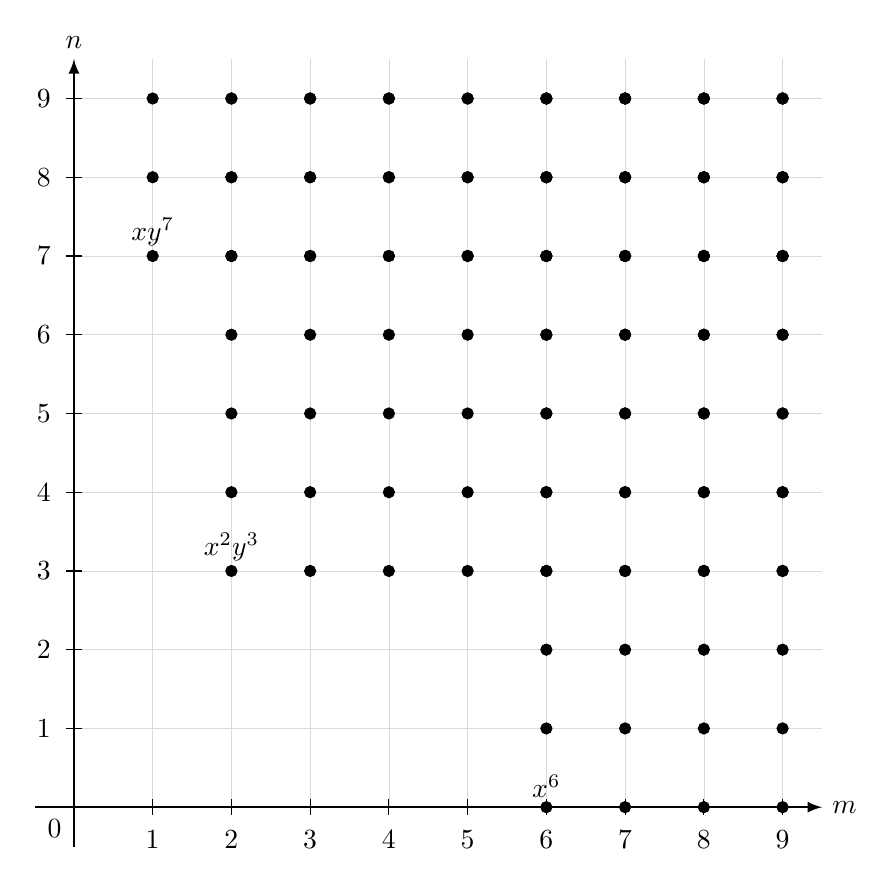
\begin{tikzpicture}[>=latex]
        \draw[step=1cm, gray!30, very thin] (0, 0) grid (9.5, 9.5);
        \draw[thick, ->] (-0.5, 0) -- (9.5, 0) node[right] {$m$};
        \draw[thick, ->] (0, -0.5) -- (0, 9.5) node[above] {$n$};
        \foreach \x in {1,2,3,4,5,6,7,8,9} {
            \draw (\x, 0.1) -- (\x, -0.1) node[below=2pt] {$\x$};
        }
        \foreach \y in {1, 2,3,4,5,6,7,8,9} {
            \draw (0.1, \y) -- (-0.1, \y) node[left=2pt] {$\y$};
        }
        \node[below left=1pt] at (0,0) {$0$};

        \draw (6, 0) node[above] {$x^6$};
        \foreach \x in {6,7,8,9} {
            \foreach \y in {0,1,2,3,4,5,6,7,8,9} {
                \filldraw (\x,\y) circle (2pt);
            }
        }

        \draw (2, 3) node[above] {$x^2y^3$};
        \foreach \x in {2,3,4,5,6,7,8,9} {
            \foreach \y in {3,4,5,6,7,8,9} {
                \filldraw (\x,\y) circle (2pt);
            }
        }

        \draw (1, 7) node[above] {$xy^7$};
        \foreach \x in {1,2,3,4,5,6,7,8,9} {
            \foreach \y in {7,8,9} {
                \filldraw (\x,\y) circle (2pt);
            }
        }
        
    \end{tikzpicture}
    \caption{Elements $x^m y^n \in \langle x^6, x^2y^3, xy^7\rangle \subseteq k[x,y]$}
    \label{fig1}
    \end{figure}
    \item[b.] Let $f \in I$ be any polynomial. When we divide $f$ by the generators of $I$, the remainder must be zero! We get 
    \[
    f = q_1 x^6+q_2 x^2y^3+q_3xy^7+r
    \]
    where no term in $r$ is divisible by any of the generators of $I$. Since $r \in I$, we must have that $r = 0$ (see Problem 8 below). Intuitively, since we can write $f = h_1(x,y)\cdot x^6 +h_2(x,y)\cdot x^2y^3+h_3(x,y)\cdot xy^7$, all monomial terms will be divisible by some generator. At each step of the division algorithm, we can only ever subtract some multiple of one the divisors, which are monomials. Since the divisors are monomials, at each step we preserve the property that every monomial term in $f$ is divisible by some generator, so we never encounter a term that we need to kick to the remainder.
\end{enumerate}
\newpage{}
\paragraph{Problem 8}
Let $I = \langle x^{\alpha(1)},\dots,x^{\alpha(s)}\rangle\subseteq k[x_1,\dots,x_n]$ be a finitely generated monomial ideal. We will show that $f \in I$ if and only if the remainder of dividing $f$ by $(x^{\alpha(1)},\dots,x^{\alpha(s)})$ is $0$. For the backwards implication (`if' direction), we have that $f = r+\sum_{i=1}^s q_i x^{\alpha(s)}$. Since $r=0$, $f$ is a $k$-linear combination of monomials $x^{\alpha(i)}$ in the ideal, so $f \in I$ (Lemma 3). 

For the nontrivial direction, let $f \in I$. By the division algorithm, we would find \[ f = r +\sum_{i=1}^s q_{\alpha(i)} x^{\alpha(i)}\]
where either $r=0$ or none of the terms in $r$ are divisible by any $\text{LT}\left(x^{\alpha(i)}\right) = x^{\alpha(i)}$. Because $f \in I$ and $x^{\alpha(i)} \in I$, we must have $r \in I$. Thus, we can write $r = \sum_i h_i \cdot x^{\alpha(i)}$ and expand with $h_i = \sum_{j} c_{ij} x^{\gamma(j)} \in k[x_1,\dots,x_n]$ to get \[
r=\sum_{i,\;j} c_{ij}x^{\alpha(i)+\gamma(j)}.
\] Thus, every monomial term in $r$ can be written as $x^{\alpha(i)+\gamma(j)}$ for some $i$ and $j$, so every monomial term is divisible by some $x^{\alpha(i)}$. If $r\ne0$, this would contradict the property of the division algorithm that no term is divisible, so $r=0$ as desired.


%We can show that at every step of the division algorithm, $\text{LT}(p)$ will be a multiple of some term of $f$. At the first step, $p=f$ and so we have the base case $\text{LT}(p) = c\cdot x^\gamma$ for some monomial term $x^\gamma$ in $f$. For the inductive step, note that if we update $p' \leftarrow p-\text{LT}(p)$, we still have the result, and if $p' \leftarrow p - x^{\alpha(i)}\cdot\text{LT}(p) / \text{LT}\left(x^{\alpha(i)}\right)$, since all our divisors are monomials we get $\text{LT}(x^{\alpha(i)}) = x^{\alpha(i)}$ so this update is the same as $p' \leftarrow p - \text{LT}(p)$. \textbf{TODO: REWRITE REWRITE JUST USE DIVISION ALGO PROPERTIES}
% Let $x^\gamma$ be any monomial term in $f$, and by Lemma 3 we have $x^\gamma \in I$ (also proven in part (b) of the problem above). Thus, there is some $1 \le i \le s$ such that $x^{\alpha(i)}$ divides $x^\gamma$ by Lemma 2. Notice that at each step of the division algorithm, $\text{LT}(p)$ will be a scalar multiple of some term $x^\gamma$ of the original $f$. (\textbf{TODO: More detail here?}) Because we have shown that all terms of $f$ are divisible by some $x^{\alpha(i)}$, our division algorithm can never encounter a term that it must kick to the remainder, so we must terminate with $r = 0$.

\end{prob}
\bigskip 




\end{flushleft}
\end{document}